\documentclass[xcolor=table]{beamer}

\usepackage[serbianc]{babel}
\usepackage{graphicx}
\usepackage{makeidx}
\usepackage{listings}
\usepackage{adjustbox}
%\usepackage[table,xcdraw]{xcolor}

\lstset{
    escapechar={|},
}

\hypersetup{unicode}
\makeindex
\usefonttheme{professionalfonts}
\usetheme{CambridgeUS}

\title{System V File System}
\author{Борисав Живановић}

\begin{document}

    \begin{frame}
        \maketitle
    \end{frame}
    
    \begin{frame}{Увод}
        \begin{itemize}
            \item До сада, били смо упознати са радом са директоријумима и фајловима из перспективе корисника
            \item Сада желимо да видимо како су ти подаци организовани на диску
            \begin{itemize}
                \item и како функционишу библиотеке са којима смо до сада приступали фајловима
            \end{itemize}
            \item Неопходно је да се подсетимо основих појмова из архитектуре рачунара и оперативних система
        \end{itemize}
    \end{frame}
    
    \begin{frame}{Шта рачунар заиста зна да ради?}
        \begin{itemize}
            \item Језик рачунара: \textbf{скуп инструкција} (енгл. ISA, Instruction Set Architecture)
            \item Аритметичке операције: \textbf{add}, \textbf{sub}, \textbf{div}, \textbf{mul}, …
            \item Померање података:
            \begin{itemize}
                \item са улазног уређаја у меморију
                \item из меморије на излазни уређај
                \item са једне меморијске локације на другу
            \end{itemize}
            \item Условно гранање: извршавање кода уколико је логички услов испуњен
        \end{itemize}
    \end{frame}
    
    \begin{frame}[allowframebreaks]{Меморијска хијерархија}
        \textit{
            Ideally one would desire an indefinitely large
            memory capacity such that any particular... word
            would be immediately available... We are... forced
            to recognize the possibility of constructing a
            hierarchy of memories each of which has greater
            capacity than the preceding but which is less
            quickly accessible.
        }

        \begin{flushright}
            \textbf{Burks, Goldstine, von Neumann} (1946)
        \end{flushright} 

        \framebreak
        
        \begin{itemize}
            \item Проблем: не постоји бесконачно брза и бесконачно велика меморија
            \item Чињеница: постоје технологије меморије које омогућавају релативно велики капацитет, по цену релативно мале брзине
            \begin{itemize}
                \item ...као и обрнуто!
                \item брзина и капацитет меморије су, по правилу, обрнуто сразмерни
            \end{itemize}
            \item Да ли је могуће добити највећи капацитет уз највећу брзину, по најмањој цени?
            \item Меморијска хијерархија нам ово \textit{донекле} омогућава
            \begin{itemize}
                \item цена: \textit{приближно} најспорија меморија
                \item брзина: \textit{приближно} најбржа меморија
            \end{itemize}
        \end{itemize}
        
        \framebreak

        \begin{figure}
            \centering
            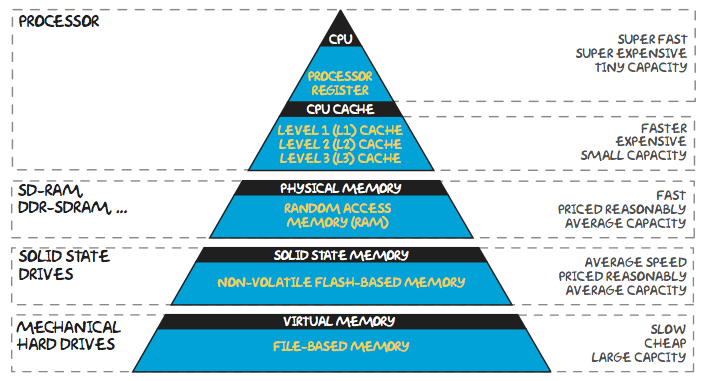
\includegraphics[width=\textwidth,height=0.7\textheight,keepaspectratio]{images/mem1.jpg}
            \label{fig:mem1}
        \end{figure}
    \end{frame}
    
    \begin{frame}{Контрола приступа у хардверу}
        \begin{itemize}
            \item Рачунар без контроле приступа би донекле био употребљив у једнокорисничком окружењу
            \begin{itemize}
                \item ...али неупотребљив у вишекорисничком
                \item чак и у једнокорисничком окружењу, одсуство изолације процеса представља велику опасност
            \end{itemize}
            \item Основне градивне блокове је неопходно имплементирати у хардверу
            \begin{itemize}
                \item софтвер можда неће бити рад да сарађује!
            \end{itemize}
            \item Кључни механизми: режими рада процесора, виртуелна меморија
        \end{itemize}
    \end{frame}
    
    \begin{frame}{Режими рада процесора}
        \begin{itemize}
            \item Привилеговани: IO, меморијске табеле, табеле прекида
            \begin{itemize}
                \item кернел
            \end{itemize}
            \item Неривилеговани: аритметичко/логичке операције, условно гранање, ограничен приступ меморији, системски позив
            \begin{itemize}
                \item кориснички софтвер
            \end{itemize}
            \item Прелазак из непривилегованог у привилеговани режим је могућ приликом прекида или системског позива
            \item Кернел одбија захтев уколико кориснички процес нема потребне привилегије и убија га
        \end{itemize}
    \end{frame}
    
    \begin{frame}[allowframebreaks]{Покретање оперативног система}
        \begin{itemize}
            \item Процесор се буди у привилегованом режиму
            \item Учитава се кернел
            \item Иницијализују се табеле прекида
            \item Иницијализују се меморијске табеле
            \item Контрола се предаје корисничким програмима, прелази се у непривилегован режим
            \item Овако подешен посредник (кернел) више није могуће уклонити или заобићи
            \begin{itemize}
                \item ...под претпоставком да нема багова у имплементацији кернела и хардвера
            \end{itemize}
        \end{itemize}
        
        \framebreak
        
        \begin{figure}
            \centering
            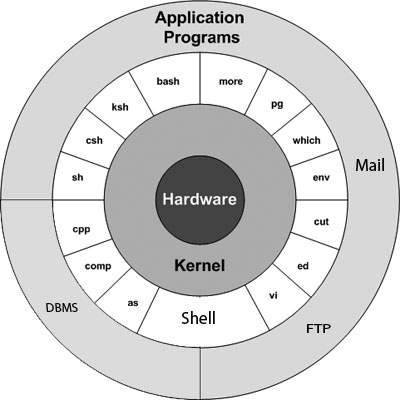
\includegraphics[width=\textwidth,height=0.8\textheight,keepaspectratio]{images/unix_architecture.jpg}
            \label{fig:unix_architecture.jpg}
        \end{figure}
    \end{frame}
    
    \begin{frame}[allowframebreaks]{Фајл систем}
        \begin{itemize}
            \item Представља формат организације података на трајном складишту
            \item Хијерархијска структура (стабло)
            \item Уводи две главне апстракције:
            \begin{itemize}
                \item \textbf{фајл}: именовани запис
                \item \textbf{директоријум}: групише друге директоријуме и фајлове
            \end{itemize}
            \item Додатно: контрола приступа фајловима
            \begin{itemize}
                \item IO инструкције се извршавају у привилегованом режиму
                \item интеракција са трајним складиштем је могућа искључиво преко системских позива
                \item систем одбија извршавање акције уколико корисник нема овлашћење
            \end{itemize}
        \end{itemize}
        
        \framebreak
        
        \begin{figure}
            \centering
            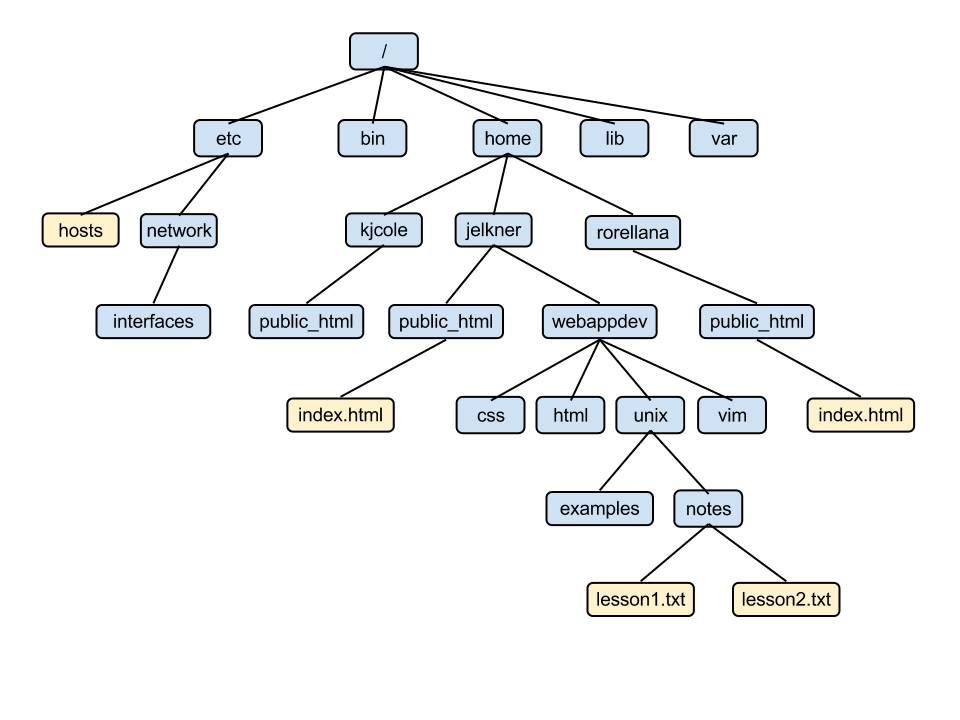
\includegraphics[width=\textwidth,height=0.8\textheight,keepaspectratio]{images/UnixDirectoryTree.png}
            \label{fig:UnixDirectoryTree.png}
        \end{figure}
    \end{frame}
    
    \begin{frame}{UNIX file API}
        \begin{itemize}
            \item fopen
            \item fread
            \item fwrite
            \item fseek
            \item fclose
        \end{itemize}
    \end{frame}
    
    \begin{frame}{Трајно складиште}
        \begin{figure}
            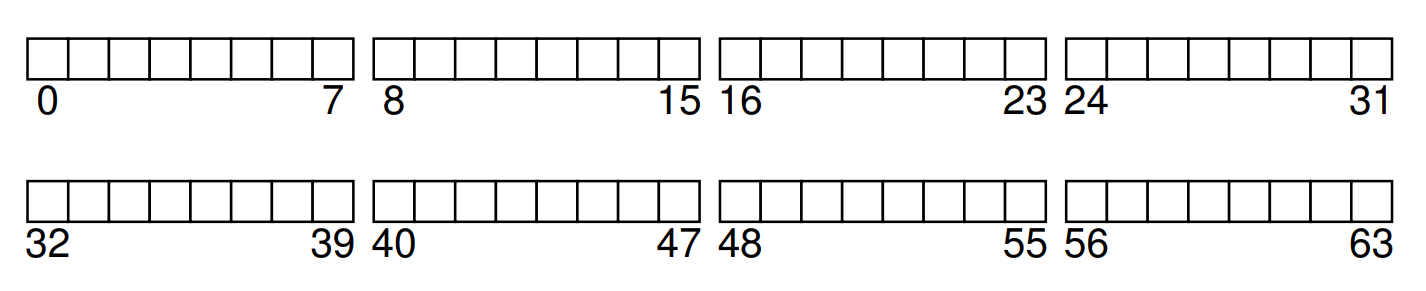
\includegraphics[width=\textwidth,height=0.8\textheight,keepaspectratio]{images/hdd_address_space.png}
            \label{fig:hdd_address_space.png}
        \end{figure}
        
        Трајно складиште можемо посматрати као \textbf{адресни простор}. Разлика у односу на радну меморију је да је најмања јединица коју
        је могуће адресирати 512 бајтова.
    \end{frame}
    
    \begin{frame}{Структура фајл система}
        \begin{figure}
            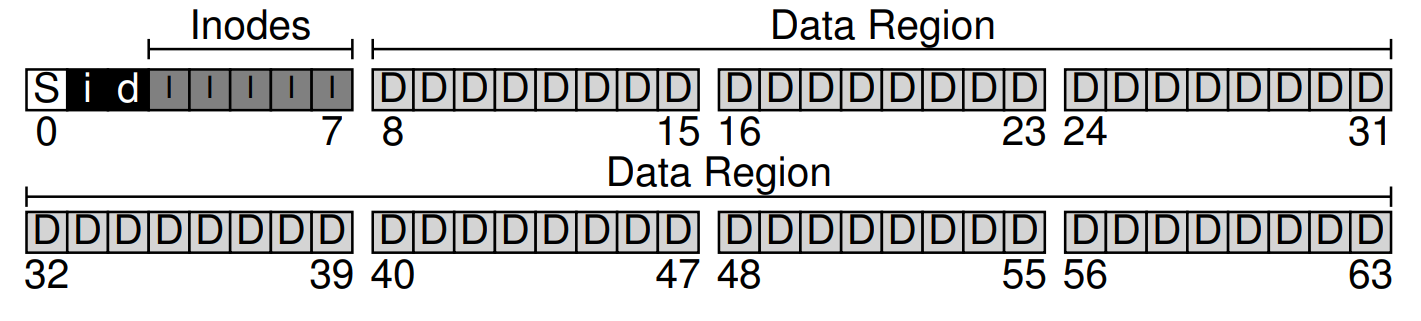
\includegraphics[width=\textwidth,height=0.8\textheight,keepaspectratio]{images/fs_structure.png}
            \label{fig:fs_structure.png}
        \end{figure}
        
        \textbf{Superblock}: метаподаци о фајл систему
        
        \textbf{Inodes}: метаподаци о садржају фајл система, један inode представља један фајл или директоријум
        
        \textbf{Data Region}: блокови који представљају садржај датотека
    \end{frame}
    
    \begin{frame}{Superblock}
        \begin{itemize}
            \item Када покушавамо да интерпретирамо садржај фајл система, неопходно је да имамо полазну тачку
            \item Садржи основне податке о фајл систему
            \begin{itemize}
                \item величину фајл система
                \item величину листе inode-ова
                \item број слободних inode-ова и data block-ова
                \item први део листе слободних data block-ова
                \item неке слободне inode-ове (налик кешу)
            \end{itemize}
        \end{itemize}
    \end{frame}
    
    \begin{frame}[allowframebreaks]{Free inode list}
        \begin{itemize}
            \item Неопходно је да знамо који inode-ови су слободни, како би могли да их искористимо за креирање фајлова/директоријума
            \item У inode листи, слободни inode-ови су означени тако што је mode = 0
            \item Додатну (кеширану) листу садржи superblock
        \end{itemize}
        
        \framebreak
        
        \begin{figure}
            \centering
            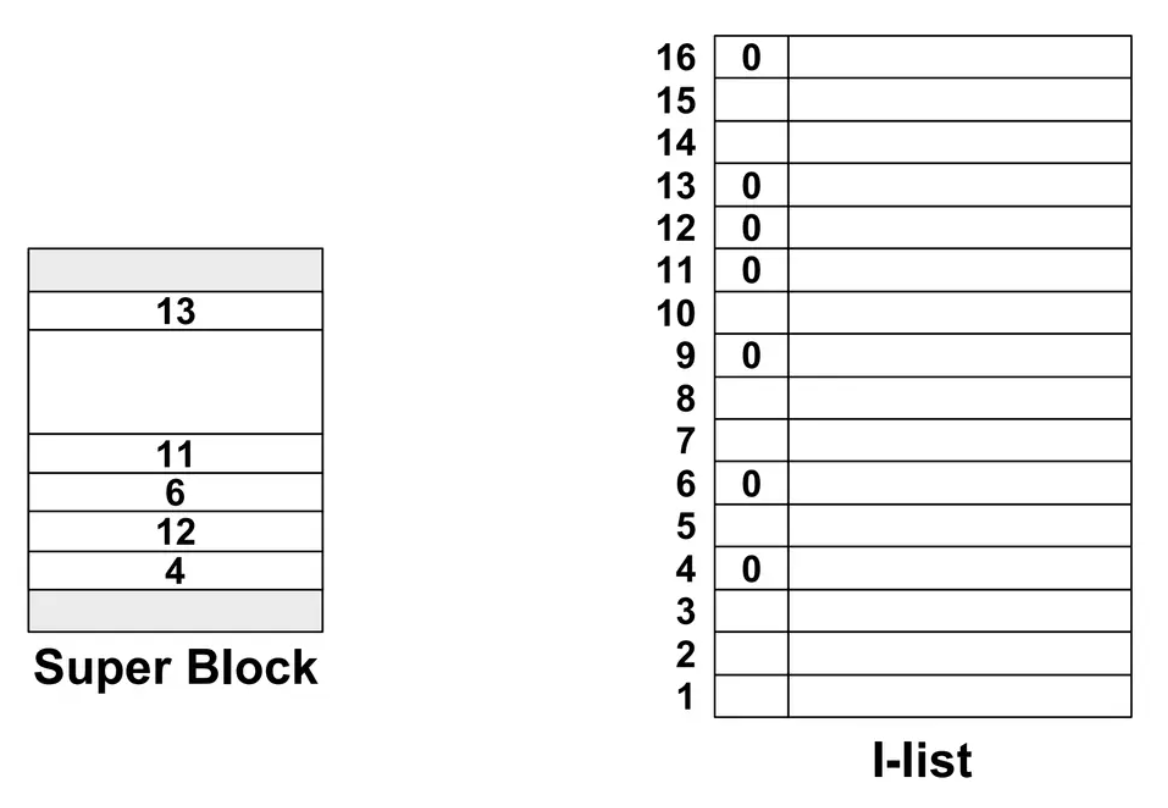
\includegraphics[width=\textwidth,height=0.8\textheight,keepaspectratio]{images/free_inode_list.png}
            \label{fig:free_inode_list.png}
        \end{figure}
    \end{frame}
    
    \begin{frame}[allowframebreaks]{Free data block list}
        \begin{itemize}
            \item Неопходно је да знамо који data block-ови су слободни, како би могли да их искористимо за чување садржаја фајлова/директоријума
            \item Први део (100 показивача) се налази у superblock-у
            \begin{itemize}
                \item уколико то није довољно да би се описао слободан простор, задњи показивач показује на листу од још 100 слободних блокова
                \item ...и тако даље, док сав слободан простор није описан
            \end{itemize}
            \item Структура налик на комбинацију array list и linked list
            \item Ослобађање data block-а изазива реконструкцију лист
        \end{itemize}
        
        \framebreak
        
        \begin{figure}
            \centering
            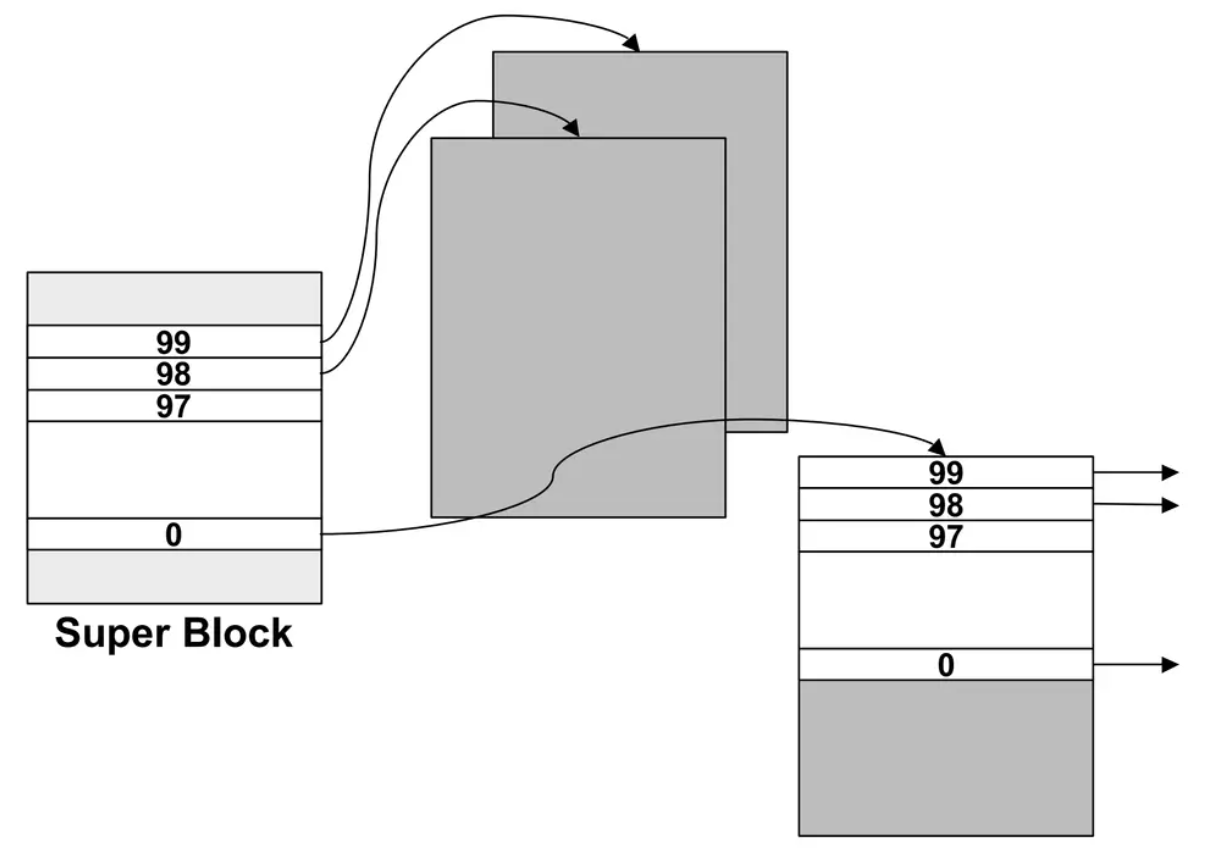
\includegraphics[width=\textwidth,height=0.8\textheight,keepaspectratio]{images/free_list.png}
            \label{fig:free_list.png}
        \end{figure}
    \end{frame}
    
    \begin{frame}[allowframebreaks]{Inode}
        \begin{itemize}
            \item Један inode (index node) представља један фајл или директоријум
            \item Уколико представљамо фајл, inode показује на блокове који чувају садржај
            \item Уколико представљамо директоријум, inode представља фајл са посебном стурктуром
            \begin{itemize}
                \item у суштини, парови (назив фајла, inode ID)
                \item и даље важе сва правила чувања обичних фајлова!
            \end{itemize}
            \item Број inode-ова ограничава број фајлова/директоријума које је могуће представити фајл системом
            \item Додатно: подаци о власништву (због контроле приступа)
        \end{itemize}
        
        \framebreak
        
        \begin{figure}
            \centering
            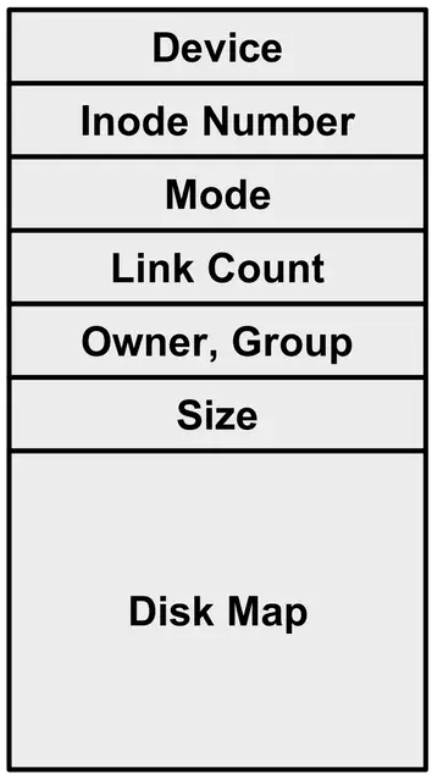
\includegraphics[width=\textwidth,height=0.8\textheight,keepaspectratio]{images/inode1.png}
            \label{fig:inode1.png}
        \end{figure}
    \end{frame}
    
    \begin{frame}[allowframebreaks]{Inode Disk Map}
        \begin{itemize}
            \item Представља асиметрично стабло
            \item Показивачи 0-9 су директни
            \begin{itemize}
                \item чувају адресу data block-a који садржи податке
            \end{itemize}
            \item Показивач 10 је индиректан
            \begin{itemize}
                \item чува адресу data block-a који садржи адресе других data block-ова
            \end{itemize}
            \item Показивач 11 је двоструко индиректан
            \item Показивач 12 је троструко индиректан
            \item Нивои индирекције су уведени због односа величине метаподатака и садржаја фајлова
            \item Број показивача ограничава величину фајла који је могуће представити у фајл систему
        \end{itemize}
        
        \framebreak
        
        \begin{figure}
            \centering
            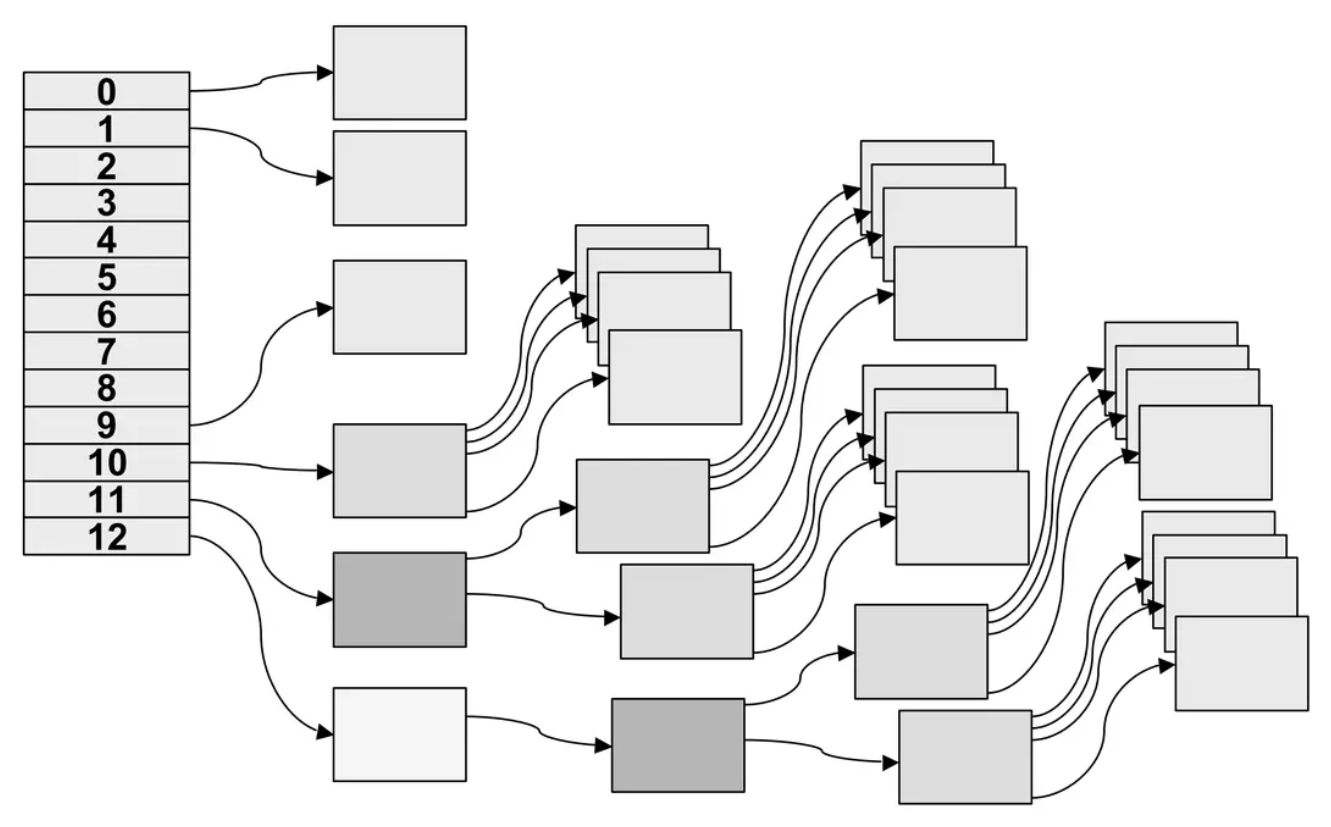
\includegraphics[width=\textwidth,height=0.8\textheight,keepaspectratio]{images/inode_data_pointers.png}
            \label{fig:inode_data_pointers.png}
        \end{figure}
    \end{frame}
    
    \begin{frame}[allowframebreaks]{Формат директоријума}
        \begin{figure}
            \centering
            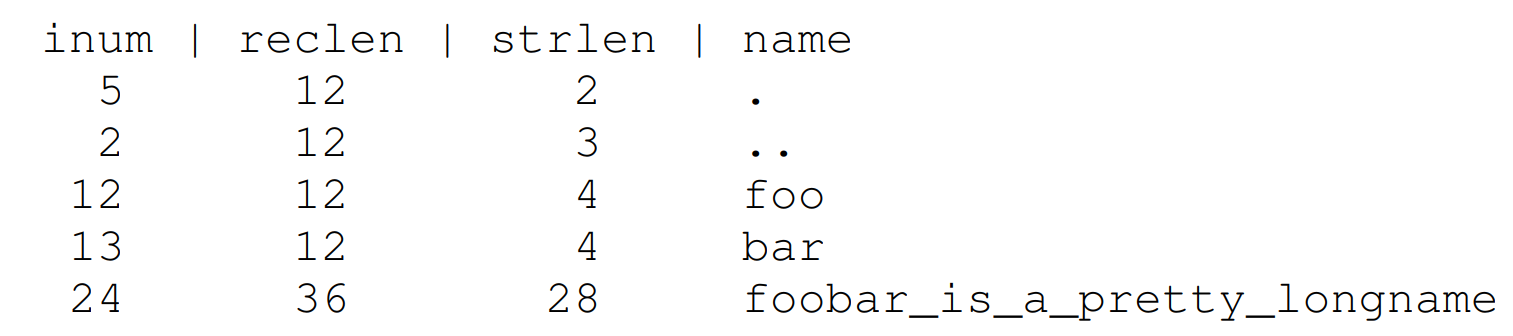
\includegraphics[width=\textwidth,height=0.8\textheight,keepaspectratio]{images/dir_layout1.png}
            \label{fig:dir_layout1.png}
        \end{figure}
        
        \framebreak
        
        \begin{figure}
            \centering
            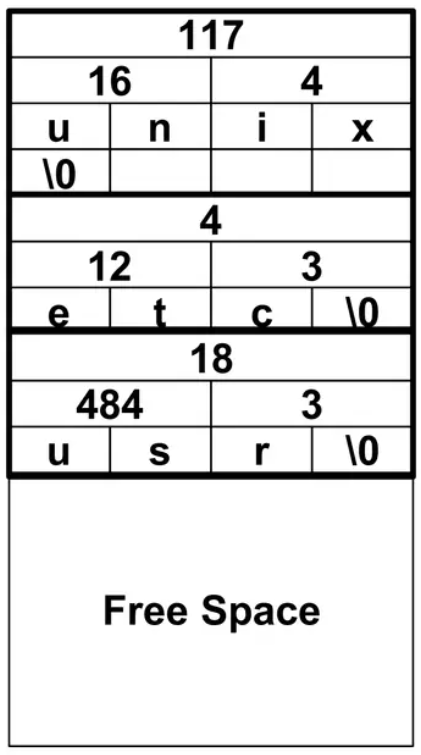
\includegraphics[width=\textwidth,height=0.8\textheight,keepaspectratio]{images/dir_layout2.png}
            \label{fig:dir_layout2.png}
        \end{figure}
    \end{frame}
    
    \begin{frame}[allowframebreaks]{Читање фајла}
        \begin{itemize}
            \item Желимо да прочитамо фајл \textbf{/foo/bar}
            \item Да би добавили садржај, потребно је наћи inode који представља \textbf{bar}
            \item Путању растављамо на делове [\textbf{/}, \textbf{foo}, \textbf{bar}]
            \item Проналазимо inode који представља \textbf{/}
            \begin{itemize}
                \item то је увек inode ID 2, проналазимо га у листи по индексу
            \end{itemize}
            \item Читамо садржај директоријума \textbf{/}, проналазимо inode који представља \textbf{bar}
            \item Читамо садржај директоријума \textbf{bar}, проналазимо inode који представља \textbf{foo}
            \item Читамо садржај фајла \textbf{foo}
            \item Уписује се време прступа у inode \textbf{foo}
        \end{itemize}
        
        \framebreak
        
        \begin{figure}
            \centering
            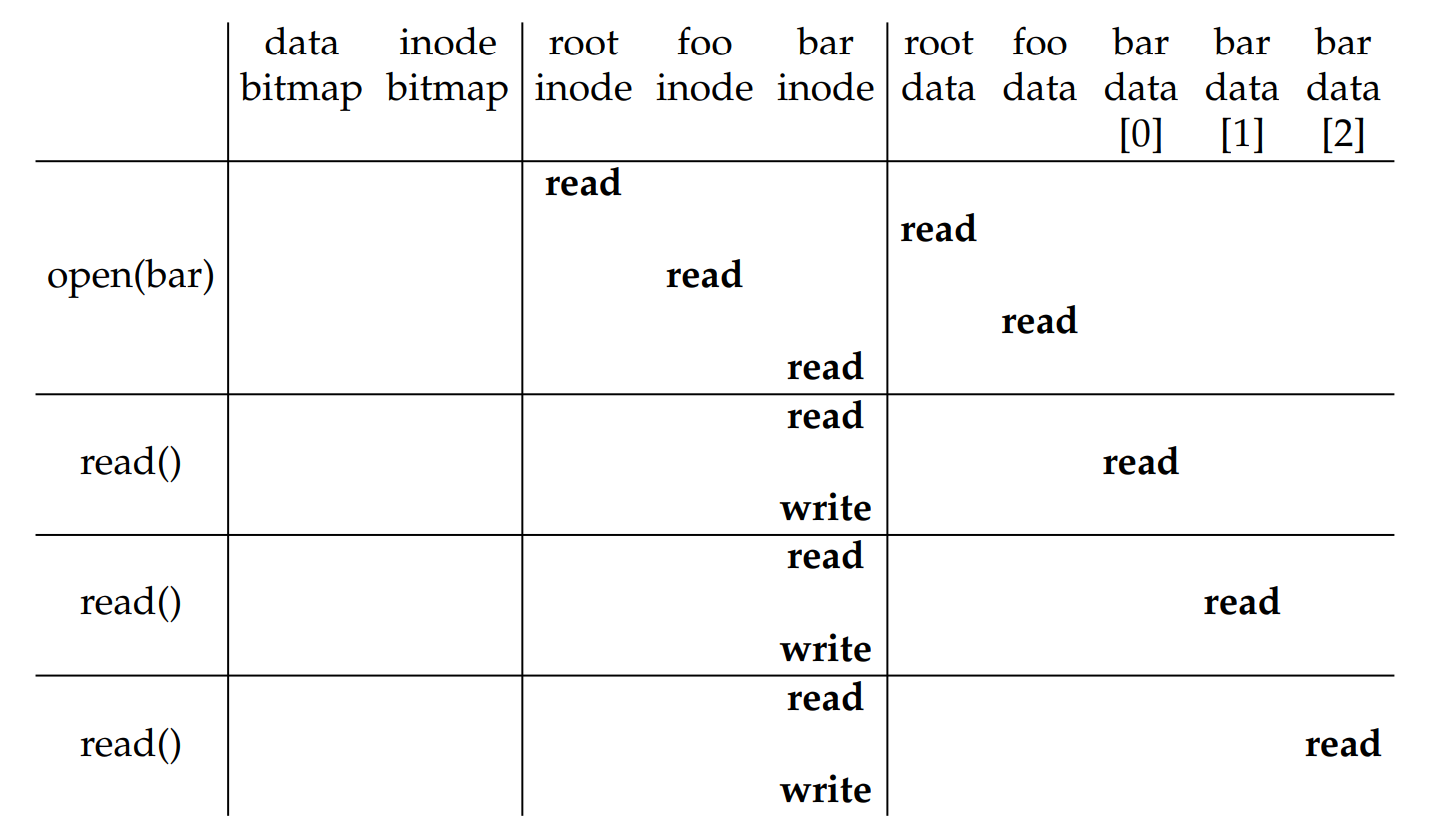
\includegraphics[width=\textwidth,height=0.8\textheight,keepaspectratio]{images/read.png}
            \label{fig:read.png}
        \end{figure}
    \end{frame}
    
    \begin{frame}[allowframebreaks]{Исписивање фајла}
        \begin{itemize}
            \item Желимо да испишемо нови фајл \textbf{/foo/bar}
            \item Проналазимо слободан inode
            \item Креирамо нови inode који ће да представља \textbf{bar}
            \item inode \textbf{bar} означавамо као заузет
            \item Проналазимо директоријум \textbf{/foo}
            \item У фајл који представља директоријум додајемо нови запис (foo, new ID)
        \end{itemize}
        
        \framebreak
        
        \begin{figure}
            \centering
            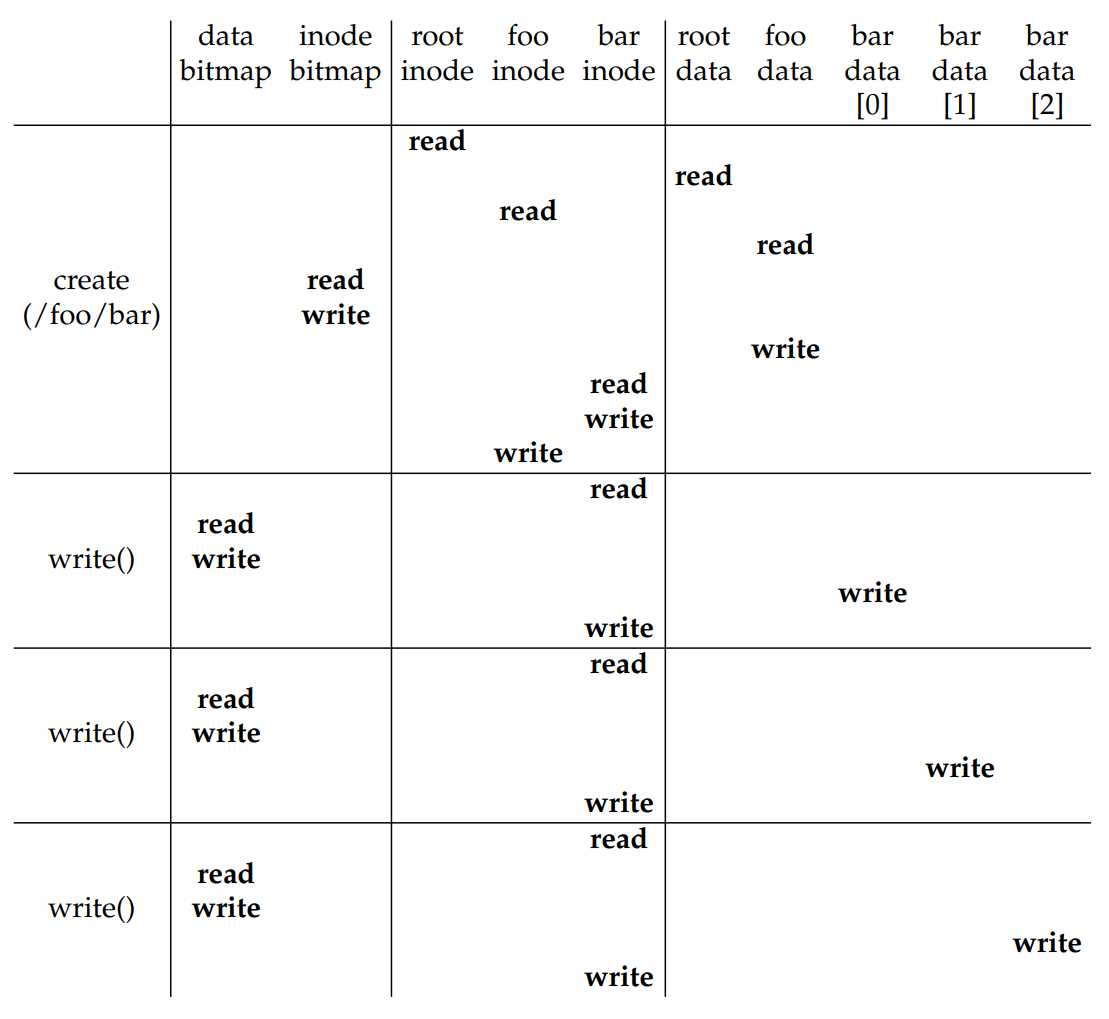
\includegraphics[width=\textwidth,height=0.8\textheight,keepaspectratio]{images/write.png}
            \label{fig:write.png}
        \end{figure}
    \end{frame}
    
    \begin{frame}{Литература}
        \begin{itemize}
            \item Operating Systems: Three Easy Pieces, Remzi H. Arpaci-Dusseau \& Andrea C. Arpaci-Dusseau
            \item File Systems, Thomas Doeppner
            \item Unix File System, Sechang (Sonny) Son
            \item Computer Organization and Design: The Hardware/Software Interface, David A. Patterson \& John L. Hennessy
            \item Системски софтвер (презентације), Иван Нејгебауер
            \item Operating Systems: Internals and Design Principles, William Stallings
            \item Preliminary Discussion of the Logical Design of an Electronic Computing Instrument
        \end{itemize}
    \end{frame}
\end{document}
